\section{Motivational Example}\label{sec:motivation}

To demonstrate both performance- and programming-related aspects of the data layout reorganization, we selected a matrix data structure, which is well-known by all scientists and programmers. Matrix is two-dimensional regular array where the individual elements are simple scalars (e.g., floats) and there are many ways how it can be stored in linear memory.

The two most typical layouts are the \emph{row-major} and \emph{column-major} formats, where the items in each row (or column, respectively) form a continuous sequence. The memory offset of item at position $[i,j]$ is computed as $i\cdot W + j$ in row-major layout, and $j*H + i$ in column-major layout, where $i$ is a zero-based index of the row, $j$ is the index of the column, and $W,H$ stand for the width and the height of the matrix respectively.

\begin{figure}
\begin{subfigure}{.19\textwidth}
    \centering
    \includegraphics[width=.9\linewidth]{figures/matrix-row-major}
    \caption{row-major}
    \label{fig:layout-row}
\end{subfigure} 
\begin{subfigure}{.19\textwidth}
    \centering
    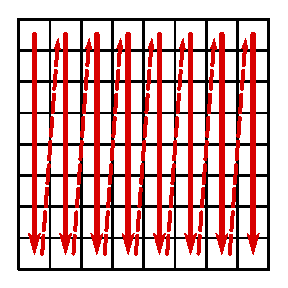
\includegraphics[width=.9\linewidth]{figures/matrix-col-major}
    \caption{col-major}
    \label{fig:layout-col}
\end{subfigure}
\begin{subfigure}{.19\textwidth}
    \centering
    \includegraphics[width=.9\linewidth]{figures/matrix-tiled}
    \caption{row-tiles}
    \label{fig:layout-tile}
\end{subfigure}
\begin{subfigure}{.19\textwidth}
    \centering
    \includegraphics[width=.9\linewidth]{figures/matrix-zcurve}
    \caption{z-curve}
    \label{fig:layout-zcurve}
\end{subfigure}
\begin{subfigure}{.19\textwidth}
    \centering
    \includegraphics[width=.9\linewidth]{figures/matrix-hcurve}
    \caption{Hilbert curve}
    \label{fig:layout-hcurve}
\end{subfigure}

\caption{Examples of common matrix layouts}
\label{fig:layout}
\end{figure}

More elaborate matrix storage layouts may promote 2D locality of the data. For instance, a matrix can be divided in tiles of $T_w \times T_h$ elements\footnote{For the sake of simplicity, we are not covering the details of handling matrix sizes that are not divisible by tile sizes.}, which are each stored as a compact block. Both the tiles and the elements within a tile may use row-major or column-major layout independently, and the tiling division can be employed on multiple levels. Ultimately, recursive subdivision leads to patterns such as the z-order curve or Hilbert curve~\cite{dai2003locality}. Examples of possible layouts are illustrated in Figure~\ref{fig:layout}.


% -----------------------------------------------------------------------------
\subsection{Performance aspects of matrix layout}\label{sec:motivation-perf}
% -----------------------------------------------------------------------------

The memory layout in combination with a particular algorithm implementation determines a memory access pattern. Different access patterns may have different performance characteristics due to properties of the selected hardware platform. The most important ones comprise:

\begin{itemize}
    \item \textbf{Hardware caches} are integral part of memory architectures, reduce the main memory latencies that are orders of magnitude higher than the latency of the registers or closest-level of caches. The optimization of their performance usually aims to minimize the amount of loads of cache lines (fixed-size cache units) from the main memory. Equivalently, programmers may aim to minimize the amount of unneeded data loaded with each cache-line by close positioning the data elements required at the same time.
    \item \textbf{Prefetching} speeds up data loading in cases when the CPU is able to detect the location of a memory access in advance, and start fetching the data before these are actually required. Most CPUs are able to reliably detect a simple sequential access pattern.
    \item \textbf{Virtual address translation} is performed with every memory access, requiring lookup in page table addresses. To speed up the lookup, a fast TLB is used as a cache. TLB misses may start to affect the performance in case a typical size of a TLB (usually hundreds of items at most) is exceeded by the amount of `active' memory pages.
\end{itemize}

In consequence, a straightforward single-pass sequential access typically yields optimal performance characteristics, conversely a completely random access pattern over large chunk of memory will prevent function of the caches and prefetching mechanism, leading to poor performance. For demonstration, we show the effects on the example of matrices, using a na\"{i}ve transpose algorithm of a square matrix impact. The algorithm might be implemented as follows:

\begin{minted}[fontsize=\scriptsize]{c++}
  for (size_t i = 0; i < N; ++i) {
    for (size_t j = i+1; j < N; ++j) {
      std::swap(m[i][j], m[j][i]);
    }
  }
\end{minted}

We can observe that both row-major and column-major layouts would be suboptimal for sufficiently large matrices. In each step, two items from the matrix are swapped. In row-major layout, the first arguments for swap (\texttt{m[i][j]}) will be accessed in optimal sequential manner, but the second ones (\texttt{m[j][i]}) will exhibit a highly strided access (two subsequent accesses are $N$ items apart) which may not be detected by prefetcher and may cause `cache spilling', as each data item is loaded with entire cache line.

Employing a z-order curve layout will mitigate the difference between row-first and column-first access, especially from the perspective of cache utilization. The row-first access pattern is only slightly worse than with the row-major layout but the column-first access is improved significantly. As a result, the algorithm may run several times to several orders of magnitude faster, depending on the platform.

Alternatively, one may utilize a different algorithm for matrix transpose. A fast approach designed for contemporary architectures is based on recursive decomposition of the matrix, where each step divides the given sub-matrix into four quadrants and transposes them in sequence. The effect on data access pattern is similar to selecting an optimal layout for the sequential algorithm, which comes at the cost of making the algorithm implementation more complex and potentially error prone.

For this reason, here we mainly aim to change the layouts of the underlying data structures, while keeping the algorithm intact in its most apprehensible form.


% -----------------------------------------------------------------------------
\subsection{Decoupling layouts from algorithms}
% -----------------------------------------------------------------------------

To make the algorithms adaptable to many layouts, we need to programmatically abstract out the implementation of all layout-specific computation, with a uniform, layout- and algorithm-agnostic interface. With matrices, we may require a method that returns a reference to an item based on $i,j$ coordinates.

In a traditional OOP-design, a matrix would be encapsulated in an object where the item accessor would be a method:
\begin{minted}[fontsize=\scriptsize]{c++}
  template<typename T = float> class Matrix {
  public:
    T& at(size_t i, size_t j) { /* ... */ }
  };
\end{minted}

For implementing different layouts, programmer might choose to inherit the methods into the class. However, that would require \texttt{at()} to be a virtual method, requiring to perform late binding upon each data item access, which is sub-optimal from the performance point of view.

A more elaborate, frequently used approach is to introduce a~policy class that governs the layout (and possibly other concerns, including memory allocation), and parametrize the matrix wrapper:

\begin{minted}[fontsize=\scriptsize]{c++}
  class RowMajor {
    static size_t offset(size_t i, size_t j, size_t W, size_t H) {
      return i*W + j;  
    }
  };

  template<typename T = float, class Layout = RowMajor>
  class Matrix {
    /* ... */
    T& at(size_t i, size_t j) {
      return _data[Layout::offset(i, j, _W, _H)];
    }
  };
\end{minted}

The policy class makes the matrix implementation both flexible (in the terms of selecting proper layout) and efficient (since the static method can be inlined by the compiler). However, several drawbacks make this solution imperfect:

\begin{itemize}
    \item The interface between the main class (i.e., \texttt{Matrix} in the previous example) and its layout policy (\texttt{RowMajor}) is created ad-hoc and is typically designed by the author of the main class. That complicates code reusability of the layout policies in potentially compatible situations (e.g., when matrix layout needs to be adopted for a structure that represents vector of points in $\mathbb{R}^d$).
    \item The interface often prevents efficient constant propagation and caching of intermediate values. For instance, the size of the matrix is passed down to \texttt{offset()} at each call, which may be suboptimal if the dimensions are compile-time constants and inter-procedural optimization is not admissible. Furthermore, accesses to items of one row in row-major layout may require unneeded repetitive re-computation of $i\cdot W$ since the policy can not predict the access pattern, and the main class cannot make any assumptions about the layout.
    \item The strong encapsulation of the data in class \texttt{Matrix}, which is considered a good-practice in general, may hinder the optimization efforts employed in performance-oriented programming. The class and algorithms that use it cannot be easily ported to GPU architectures for instance, and impose a data interface that may be detrimental for certain more complex access methods (such as block-wise loads with SIMD or offloading parts of the matrix to shared memory of a GPU).
    \item The encapsulation provided by the main class also complicates integration in larger data structures. For example, a collection of matrices may benefit from a memory layout where the matrices are interleaved.
\end{itemize}

% -----------------------------------------------------------------------------
\subsection{First-class indexing structures}
\label{subsec:fstclass}
% -----------------------------------------------------------------------------

\begin{listing}[h]
    \vspace{-10pt}
    \inputmintedcpp{noarr/code-snippets/noarr_transpose.cpp}
    \vspace{-20pt}
    \caption{The example of matrix transpose that employs first-class layout structures implemented in \Noarr{} library.}
    \label{lst:demo-noarr}
\end{listing}

To improve upon the drawbacks mentioned in previous section, we introduce layouts as first-class structures, which provide the required indexing (offset computation) operations, expose the details of the layout to the programs, and can be easily composed to form complex layouts from smaller primitive `building blocks' having the type of the layout flexible and easily constructible from pre-implemented primitives. The main features are demonstrated in Listing~\ref{lst:demo-noarr}, which shows the matrix transpose algorithm implemented with the first-class layout structures.

In the example, the layout type (row-major in this case) is constructed on line $30$ from the \Noarr{} primitives for vectors of items. These are connected to a sequence of matrices on line $31$. The structure has explicitly named dimensions, here marked with characters\footnote{Any type convertible to integer can be used for dimension names, including enumerations.}, which makes the access more mnemonic for the programmers (as seen on line $5$). The naming of the dimensions is entirely processed at compile-time by the C++ compiler, creating no overhead in the resulting code.

The matrix sequence layout object is created on line $33$ to provide dynamic sizes to a statically defined layout type. This is achieved by instantiating \texttt{matrix\_sequence} type and by applying \texttt{set\_length} functions to each dimension specified by a character literal. On line $37$, the layout object is converted into a \texttt{bag} structure that, for convenience, explicitly binds the layout and a data pointer together, creating a work-alike of common data objects. The actual allocation of the memory is not shown in the example, but may be executed by a helper function that determines the required size from the layout object. Line $37$ demonstrates a `partial' indexing, fixing arbitrary dimensions of the layout structure, so that the \texttt{transpose()} function can only work with a single pre-selected matrix. This corresponds to creation of arbitrary (even irregular) array slices.

The structure object is passed to functions in two parts --- as a value (first-class parameter) and also as type (template parameter). This way, both static data (such as the size and type of the `scalar' contents, and static sizes of arrays) and dynamic data (sizes of the vectors) are visible to a compiler.

The layout structure provides additional methods to help with various indexing scenarios. For instance, the \texttt{shift} method (lines 24 and 25) creates a copy of the layout structure with shifted origin (i.e., with explicit offsets embedded), simplifying the implementation of divide-and-conquer recursive pattern used in the transpose algorithm. The explicit dereferencing of the \texttt{bag} structure (the \texttt{at} method at line 5) combines computation of the offset from the layout and adding the offset to the stored pointer.

In the following sections, we detail the implementation and analyze the key benefits of this approach.
